% !TeX root = ../economia.tex
\chapter{Impresa}

\section{Definizione giuridica}

\subsection{Requisiti di un'impresa}
Per essere considerata un'\gls{impresa}, un'attività deve essere:
\begin{itemize}
    \item economica: l’output deve poter essere oggetto di \emph{scambio} su un 
    mercato (deve avere un valore \emph{economico})
    \item professionale: svolta abitualmente, ma non necessariamente, con
    \emph{continuità temporale in esclusiva} da un \gls{imprenditore} (ma è
    possibile delegare la gestione dell’\gls{impresa})
    \item organizzata: l’impresa ha una sua organizzazione, struttura che
    consente una \emph{gestione coordinata delle risorse} (umane, finanziarie,
    tecnologiche). L’imprenditore organizza liberamente l’impresa.
\end{itemize}

\section{Cosa fa l'impresa}

Un impresa utilizza come \emph{input} beni e servizi per \emph{trasformarli},
mediante delle \emph{risorse} (impianti, macchinari, personale, conoscenze
tecnologiche, brevetti) in \emph{output} da vendere ai \emph{consumatori finali}
o ad \emph{altre imprese}. L'obiettivo di un impresa è \emph{generare valore},
cioè un \gls{utile}, per gli \glspl{shareholder}. Altri obiettivi sono la
riduzione dei costi, l'aumento delle quote di mercato, il miglioramento della
qualità del prodotto, l'innovazione, l'ingresso in nuovi mercati\dots

\section{Responsabilità Sociale d'Impresa (RSI)}
La Responsabilità Sociale d’impresa (RSI) o Corporate Social Responsibility
(CSR) è ``la responsabilità delle imprese per gli impatti che hanno sulla
società''.

\subsection{Principi della RSI}
\begin{itemize}
    \item \emph{sostenibilità}: uso consapevole ed efficiente delle risorse
    ambientali in quanto beni comuni, capacità di valorizzare le risorse umane
    e contribuire allo sviluppo della comunità locale in cui l’azienda opera,
    capacità di mantenere uno sviluppo economico dell’impresa nel tempo.
    \item \emph{volontarietà}: come azioni svolte oltre gli obblighi di legge.
    \item \emph{trasparenza}: ascolto e dialogo con gli \glspl{stakeholder}.
    \item \emph{qualità}: in termini di prodotti e processi produttivi.
    \item \emph{integrazione}: visione e azione coordinata delle varie attività.
    di ogni direzione e reparto, a livello orizzontale e verticale, su obiettivi
    e valori condivisi.
\end{itemize}

\section{Rischio d'impresa}
Il \gls{rischio} è l'impossibilità di prevedere con certezza gli esiti futuri delle decisioni
in merito alle attività dell’impresa (``probabilità di un evento e delle sue
conseguenze'')

\subsection{Fattori di rischio}
\begin{itemize}
    \item \emph{Tempo}: l'imprenditore prende oggi decisioni i cui risultati si
    vedranno domani (\emph{mancano} alcune informazioni necessarie a decidere).
    \item \emph{Contesto dinamico e mutevole}: domanda, preferenze dei
    consumatori, numero e tipologia di concorrenti, tecnologie, condizioni di
    accesso al credito, etc. sono variabili nel tempo.
    \item \emph{Rigidità strutturale}: l’impresa ha un’organizzazione non
    immediatamente modificabile in risposta all’ambiente (per esempio, in caso
    di riduzione della domanda non sempre è possibile licenziare il personale).
\end{itemize}

L'imprenditore si assume il rischio d'impresa, che non è necessariamente una
fattore negativo: così come risponde delle perdite, si appropria dei guadagni.

\section{Nascita di un'impresa}
È conveniente, dopo l'idea iniziale di un'impresa, usare un \gls{bizmodel} per
descrivere le logiche con cui un organizzazione crea, distribuisce e raccoglie
valore.

\subsection{Business Model Canvas}

\begin{figure}[h]
    \centering
    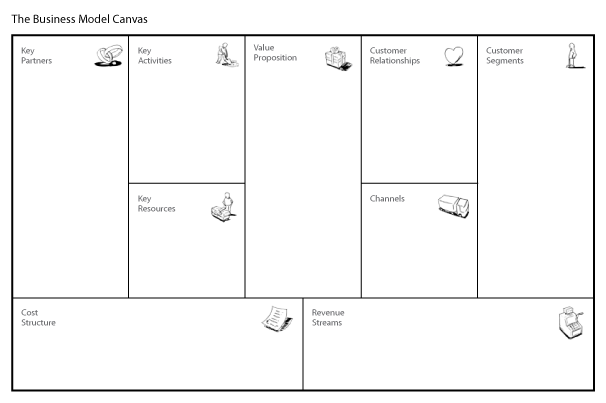
\includegraphics[width=10cm]{business_model_canvas.png}
\end{figure}

\begin{enumerate}
    \item Segmenti di clientela
    \begin{itemize}
        \item Per chi stiamo creando valore?
        \item Chi sono i nostri clienti più importanti?
    \end{itemize}
    \item Proposte di valore
    \begin{itemize}
        \item Quali problemi dei nostri clienti stiamo risolvendo?
        \item Quali bisogni dei nostri clienti stiamo soddisfacendo?
        \item Cosa lega i nostri prodotti e servizi a ciascun segmento di
        clienti?
    \end{itemize}
    \item Canali
    \begin{itemize}
        \item Attraverso quali canali possiamo raggiungere i nostri clienti? 
        \item Quali sono i canali che funzionano meglio? 
        \item Quali sono i canali meno costosi?
    \end{itemize}
    \item Relazioni con i clienti
    \begin{itemize}
        \item Che tipo di relazione ciascun segmento di clienti si aspetta di
        stabilire e mantenere con noi?
        \item Cosa occorre fare per stabilire queste relazioni?
        \item Quanto costa stabilire e mantenere queste relazioni?
    \end{itemize}
    \item Flussi di ricavi
    \begin{itemize}
        \item Cosa sono disposti a pagare i clienti? 
        \item Come preferirebbero pagare i clienti? 
        \item Quanto ciascun flusso di ricavi contribuisce ai ricavi totali?
    \end{itemize}
    \item Risorse chiave
    \begin{itemize}
        \item Quali risorse occorre possedere per poter creare valore? 
        \item Quali altre risorse sono necessarie?
    \end{itemize}
    \item Attività chiave
    \begin{itemize}
        \item Quali attività è indispensabile svolgere per creare valore?
    \end{itemize}
    \item Partner chiave
    \begin{itemize}
        \item Chi sono i nostri partner più importanti?
        \item Chi sono i fornitori più importanti?
        \item Quali risorse forniscono i nostri partner? 
        \item Quali attività svolgono i nostri partner?
    \end{itemize}
    \item Struttura di costo
    \begin{itemize}
        \item Quali sono i principali costi del modello
        di business?
        \item Quali risorse chiave sono più costose?
        \item Quali attività chiave sono più costose?
    \end{itemize}
\end{enumerate}

\subsection{Business Plan}

Il \gls{bizplan} contiene informazioni su:
\begin{itemize}
    \item Il \emph{prodotto o il servizio} che si intende offrire
    \item Il \emph{mercato} in cui l’impresa andrà ad operare
    \item La \emph{strategia} e l’implementazione della stessa
    \item Il \emph{gruppo dirigente}
    \item Le \emph{previsioni finanziarie}
\end{itemize}

\subsection{Fonti di finanziamento}

In linea di principio non serve un capitale proprio, tuttavia l’imprenditore
potrebbe raccogliere capitale da soci esterni (capitale di rischio) e/o credito
(capitale di debito) sulla base della sua idea di business.

La presenza di capitale proprio dei fondatori garantisce i creditori
da rischio di insolvenza e segnala credibilmente il valore dell’idea di
business a finanziatori esterni.

Per sostenere la crescita è necessario raccogliere capitale da finanziatori
esterni specializzati:
\begin{itemize}
    \item Banche
    \item Venture Capitalists
    \item Business Angels
    \item Crowdfunding
    \item Sussidi pubblici
\end{itemize}

\section{Morte di un'impresa}
L’impresa ha durata indefinita, infatti non muore con l’imprenditore, ma
rischia però di ``morire'' se non realizza profitti e dunque non riesce a
remunerare i fattori produttivi.

\subsection{Tipologie}

\begin{itemize}
    \item \emph{Fallimento (scioglimento coatto)}: l’impresa è sciolta per
    ordine del tribunale, i suoi beni vengono venduti
    \item \emph{Liquidazione (scioglimento volontario)}: vendita volontaria dei beni decisa dai
    soci. La ``morte'' per liquidazione non sempre ha un’accezione negativa.
    \item \emph{Acquisizione/Fusione}: l’impresa viene assorbita da un'altra
    impresa. La ``morte'' per fusione ha spesso un'accezione positiva.
\end{itemize}

\section{Tipologie di imprese}
\begin{enumerate}
    \item Proprietà
    \begin{itemize}
        \item \emph{Proprietà pubblica}: il proprietario è un ente pubblico
        (es: lo Stato)
        \item \emph{Proprietà privata}
    \end{itemize}
    \item Obiettivo
    \begin{itemize}
        \item \emph{Profit}: l’obiettivo principale è il profitto
        \item \emph{No profit}: l’obiettivo è uno scopo alternativo, spesso
        socialmente rilevante
    \end{itemize}
    \item Dimensione
    \begin{itemize}
        \item \emph{Grandi imprese}: addetti $\ge 250$ e fatturato $> 50$ \textsc{mil} \euro
        \item \emph{Medie imprese}: addetti $50-249$ e fatturato $10-50$ \textsc{mil} \euro
        \item \emph{Piccole imprese}: addetti $< 50$ e fatturato $< 10$ \textsc{mil} \euro
        \item \emph{Microimprese}: addetti $< 10$ e fatturato $\le 2$ \textsc{mil} \euro
    \end{itemize}
    \item Tipologia di output
    \begin{itemize}
        \item \emph{Beni materiali}
        \begin{itemize}
            \item Imprese agricole: producono beni con processi naturali legati 
            alla terra
            \item Imprese industriali/manifatturiere: compiono trasformazioni
            tecniche dei beni
        \end{itemize}
        \item \emph{Servizi}
        \begin{itemize}
            \item Imprese di trasporto e telecomunicazioni
            \item Distribuzione di energia elettrica, gas, acqua
            \item Negozi
            \item Banche
            \item Assicurazioni
        \end{itemize}
    \end{itemize}
    \item Numero di output
    \begin{itemize}
        \item \emph{Monoprodotto}: imprese che producono/vendono un solo prodotto
        \item \emph{Diversificate}: imprese che producono/vendono vari prodotti/servizi
        da qualche punto di vista imparentati tra loro
        \item \emph{Conglomerali}: imprese che producono/vendono vari prodotti/servizi
        poco imparentati tra loro. Spesso esiste un core business
        (prodotto/servizio ritenuto più importante)
    \end{itemize}
    \item Consumatore
    \begin{itemize}
        \item \emph{Wholesale (all’ingrosso)}: imprese che producono e vendono prodotti
        intermedi ad altre imprese che, a loro volta, li utilizzano nel loro processo
        produttivo
        \item \emph{Retail (al dettaglio)}: imprese che vendono il prodotto al consumatore in
        un mercato finale
    \end{itemize}
    \item Localizzazione delle attività produttive
    \begin{itemize}
        \item \emph{Multinazionali}: hanno interessi economici e attività produttive in più di
        una nazione
        \item \emph{Nazionali}
    \end{itemize}
\end{enumerate}

\section{Forme giuridiche}

\subsection{Imprese individuali}
Sono costituite da un'\emph{unica persona fisica}.

Il titolare (\gls{piccoloimpr}) ha \gls{respill} delle obbligazioni dell'impresa con tutto il patrimonio personale.

È tipica di attività come: commercialista, architetto, ingegnere, medico,
consulente di vario genere\dots

\subsubsection{Impresa familiare}
È un'estensione dell’impresa individuale, quando l’imprenditore
si avvale in modo continuativo della prestazione lavorativa dei familiari
(parentela fino al $3^o$ grado e affinità fino al $2^o$ grado).

\proandcons{
    Semplicità nella costituzione e lo scioglimento dell'impresa.
    Non è richiesto il versamento del capitale

    Pochi obblighi contabili
    
    Autonomia e velocità decisionale
}{
    \Gls{respill}

    In caso di forti guadagni le imposte crescono a causa delle aliquote
    progressive previste dall'Irpef
}


\subsection{Imprese collettive}

\subsubsection{Società di persone}

\paragraph{Società semplice (s.s.)} Riservata ad \emph{attività economiche non commerciali}
(attività agricole e per la gestione di patrimoni immobiliari).

\paragraph{Società in nome collettivo (s.n.c.)} Può esercitare sia attività di
impresa commerciale, sia attività economiche non commerciali.

\paragraph{Società in accomandita semplice (s.a.s.)} Si distingue tra:
\begin{itemize}
    \item Soci accomandatari: si assumono in forma illimitata e solidale le
    responsabilità connesse all'esercizio dell'impresa
    \item Soci accomandanti: affidano in gestione i loro capitali ad altri soci e
    sono responsabili solo del capitale conferito
\end{itemize}

\proandcons{
    Costituzione e tenuta della contabilità relativamente semplici
    
    Procedure burocratiche, fiscali, contabili e tributarie minime
    
    Non è obbligatorio il versamento di un capitale minimo da parte dei
    soci (l’importo è stabilito dal contratto sociale)
}{
    Responsabilità illimitata (a parte accomandanti della s.a.s.) e solidale.
    Se un socio non adempie, il debito dovrà essere saldato dagli altri.

    Minore autonomia decisionale, problemi di coordinamento 
}

\subsubsection{Società di capitali}

\paragraph{Società a responsabilità limitata (s.r.l.)}
\begin{itemize}
    \item Capitale sociale (ossia la proprietà) è diviso in quote
    \item Nell’assemblea dei soci si vota per la quota posseduta
    \item Capitale minimo: 10.000 \euro
\end{itemize}

\paragraph{Società a responsabilità limitata semplificata (S.r.l.s.)}
\begin{itemize}
    \item Forma di s.r.l. recentemente introdotta (2012) dalla legislazione per
    favorire l’imprenditorialità
    \item Capitale minimo: 1 \euro
    \item Capitale massimo: 9.999,99 \euro
    \item Modello standard dell’atto di costituzione della società, per la stipula
    dell'atto costitutivo non sono dovuti onorari notarili
\end{itemize}

\paragraph{Società per azioni (s.p.a.)}
\begin{itemize}
    \item Il patrimonio sociale è costituito da azioni
    \item Le azioni sono quote di partecipazione liberamente trasferibili
    \item Possibile quotazione in Borsa
    \item Capitale minimo: 50.000 \euro
\end{itemize}

\paragraph{Società in accomandita per azioni (s.a.p.a.)}
\begin{itemize}
    \item I soci si distinguono in accomandatari e accomandanti
\end{itemize}

\proandcons{
    Responsabilità limitata
    
    Gestione può essere affidata anche ai non soci
    
    Tassazione sulle imprese
    
    Utili possono essere distribuiti ai soci nei momenti fiscalmente più
    convenienti
    
}{
    Adempimenti burocratici e fiscali sono numerosi e complessi (es.
    contabilità ordinaria)
    
    Obbligatorio il conferimento di capitale iniziale

    Maggiori obblighi di trasparenza e di governance
}

\subsubsection{Società cooperative}

\begin{itemize}
    \item Imprese che pur svolgendo un’attività economica non hanno l’obiettivo di
    distribuire utili significativi in capo ai soci
    \item Devono reinvestire i profitti nell’attività imprenditoriale
    \item Qualora dette imprese non dovessero rispettare questi requisiti perderebbero
    il diritto alle importanti agevolazioni fiscali di cui possono beneficiare
    \item Si distinguono in società cooperative a \gls{respill} e) società
    cooperative a \gls{resplim}
\end{itemize}

\subsubsection{Startup innovative}
Dal 2012, esiste una nuova tipologia d'impresa, le \emph{startup innovative}.

\paragraph{Requisiti}

\begin{itemize}
    \item  Essere attive da meno di 5 anni
    \item Avere sede principale in Italia, o in altro Paese membro dell’Unione Europea, purché ci sia una
    sede produttiva o una filiale in Italia
    \item Avere un fatturato annuo inferiore a 5 milioni di euro
    \item Non distribuire utili
    \item Non essere costituite da fusione, scissione societaria o a seguito di cessione di azienda o di ramo
    di azienda
    \item Sviluppare, produrre e commercializzare prodotti o servizi innovativi ad \emph{alto valore tecnologico},
    ed essere in possesso di almeno uno dei tre seguenti criteri:
    \begin{itemize}
        \item Almeno il 15\% del maggiore tra fatturato e costi annui è ascrivibile ad attività di ricerca e
        sviluppo
        \item La forza lavoro complessiva è costituita per almeno 1/3 da dottorandi, dottori di ricerca o
        ricercatori, oppure per almeno 2/3 da soci con laurea magistrale
        \item L’impresa è titolare, depositaria o licenziataria di un brevetto registrato
    \end{itemize}
\end{itemize}

\paragraph{Agevolazioni}

\begin{itemize}
    \item Agevolazioni per startup innovative:
    \item Esonero pagamento dei diritti camerali annuali e imposte di bollo
    \item Gestione societaria flessibile: l’atto costitutivo delle startup innovative costituite in
    una SRL può prevedere categorie di quote che non attribuiscono diritti di voto o che ne
    attribuiscono in misura non proporzionale alla partecipazione
    \item Regime speciale per le perdite: 2 anni (al posto di 1) di tempo per il ripianamento
    delle perdite superiori ad un terzo del capitale
    \item Assunzioni del personale: contratti a tempo determinato dalla durata minima di 6
    mesi a massimo 36 mesi con rinnovo, stipendi flessibili, ecc..
    \item Incentivi fiscali per le persone fisiche e giuridiche che investono nella startup
    \item Equity crowdfunding
    \item Accesso facilitato e gratuito al credito del Fondo di Garanzia per le Piccole e Medie
    Imprese (garanzia del Governo fino a coprirne l'80% del credito erogato dalla banca)
    \item Esonero dalla procedura di fallimento aziendale e possibilità per l'imprenditore di
    intraprendere un nuovo progetto in tempi brevi
\end{itemize}
